\documentclass[a4paper, 10pt, twocolumn]{article}
\usepackage{cellspace, graphicx, makecell}
\usepackage{graphicx} % Required for inserting images
\usepackage[utf8x]{inputenc}
\usepackage[english,russian]{babel}
\usepackage{cmap}
\usepackage[left=1cm,right=1cm,
    top=1cm,bottom=2cm]{geometry}
\usepackage{paracol}
\usepackage{multicol}
\usepackage{amsmath}
\usepackage{lipsum}
\usepackage{vwcol}
\usepackage{float}

% Установка размера формул
\DeclareMathSizes{10}{10}{10}{10}   % Для основного текста размером 10pt

\title{Лабораторная работа 1.4.8 \\ Измерение модуля Юнга стержней методом акустического резонанса.}
\author{Матвей Галицын \\ Б01-411}
\date{November 28, 2024}

\setlength{\columnseprule}{0.1pt}
\setlength{\columnsep}{3em}

\begin{document}
\maketitle
\newpage{}
\section{Введение}
\textbf{Цель работы:} исследовать явление акустического резонанса в тонком стержне; измерить скорость
распространения продольных звуковых колебаний в тонких стержнях из различных материалов и различных 
размеров; измерить модули Юнга различных материалов.\\
\textbf{В работе используются:} генератор звуковых частот, частотомер, осциллограф, электромагнитные 
излучатель и приёмник колебаний, набор стержней из различных материалов.

\section{Теоретическая сведения}
\subsection{Акустические волны в стержне}
Основной характеристикой упругих свойств твёрдого тела является его модуль Юнга $E$. Согласно закону 
Гука, если к элементу среды приложено некоторое механическое напряжение $\sigma$, действующее вдоль 
некоторой оси $x$ (напряжения по другим осям при этом отсутствуют), то в этом элементе возникнет 
относительная деформацию вдоль этой же оси
$\varepsilon = \Delta x/x_0$ , определяемая соотношением
\begin{equation}
\sigma = \varepsilon \cdot E
\end{equation}
Если с помощью кратковременного воздействия в некотором элементе
твёрдого тела создать малую деформацию, она будет далее распростра-
няться в среде в форме волны, которую называют акустической или звуко-
вой. Распространение акустических волн обеспечивается за счёт упругости
и инерции среды. Волны сжатия/растяжения, распространяющиеся вдоль
оси, по которой происходит деформация, называются продольными. Как
будет строго показано далее, скорость $u$ распространения продольной аку-
стической волны в простейшем случае длинного тонкого стержня опреде-
ляется соотношением
\begin{equation}
u = \sqrt{\frac{E}{\rho}}
\end{equation}
где $\rho$ — плотность среды.
Заметим, что размерность модуля Юнга $E$ равна [Н/м$^2$] и совпадает с
размерностью механического напряжения (или давления). Характерные
значения модуля Юнга металлов лежат в диапазоне $E\sim$ 1010 ÷ 1012 Па, так
что при плотности $\rho\sim$ 104 кг/м3 характерные значения скорости звука в
твёрдых телах составляют $u\sim$ 103 - 104 м/с.
В общем случае звуковые волны в твёрдых телах могут быть не только
продольными, но и поперечными — при этом возникает деформация сдвига
перпендикулярно распространению волны. Кроме того, описание распространения волн в неограниченных средах осложняется тем
обстоятельством, что при отличном от нуля коэффициенте Пуассона напряжение вдоль одной из осей вызывает деформацию не только в продольном,
 но и в поперечном направлении к этой оси. Таким образом, общее
описание звуковых волн в твёрдых телах — относительно непростая задача.
В данной работе мы ограничимся исследованием наиболее простого случая
упругих волн, распространяющихся в длинных тонких стержнях.
Рассмотрим стержень постоянного круглого сечения, радиус $R$ которого
много меньше его длины $L$. С точки зрения распространения волн стержень
можно считать тонким, если длина $\lambda$ звуковых волн в нём велика по сравнению
 с его радиусом: $\lambda R$. Такая волна может свободно распространяться только вдоль стержня, поэтому можно считать, что стержень испытывает
 деформации растяжения и сжатия только вдоль своей оси (заметим,
что в обратном пределе коротких волн $\lambda R$ стержень следует рассматривать как безграничную сплошную среду). Если боковые стенки тонкого
стержня свободны (т.е. стержень не сжат с боков), то его деформации описывается законом Гука в форме (1), и, следовательно, его упругие свойства
определяются исключительно модулем Юнга среды.
Акустическая волна, распространяющаяся в стержне конечной длины $L$,
испытает отражение от торцов стержня. Если при этом на длине стержня
укладывается целое число полуволн, то отражённые волны будут складываться в фазе с падающими, что приведёт к резкому усилению амплитуды
их колебаний и возникновению акустического резонанса в стержне. Измеряя соответствующие резонансные частоты, можно определить скорость
звуковой волны в стержне и, таким образом, измерить модуль Юнга материала стержня. Акустический метод является одним из наиболее точных
методов определения упругих характеристик твёрдых тел.
\subsection{Установка. Резонансная частота}
\begin{figure}[h]
    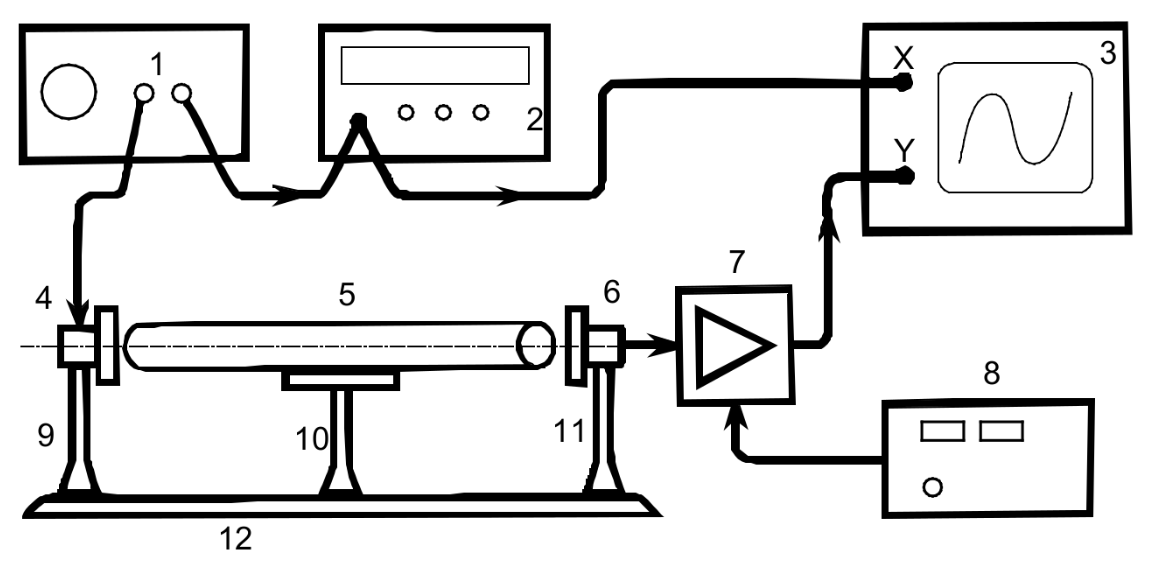
\includegraphics[width=1\linewidth]{images/installation.png}
    \begin{center}
        \caption{cхема установки. \\ 1 - генератор звуковой частоты; 2 - частотомер; 3 - осциллограф; 4 - 
    электромагнит-возбудитель; 5 - образец; 6 - электромагнит-приемник; 7 - усилитель звуковой частоты;
     8 - блок питания усилителя; 9, 11 - стойки крепления электромагнитов; 10 - стойка крепления об
     разца; 12 - направляющая;}
    \end{center}
\end{figure} 

\par Схема экспериментальной установки приведена на рис. 1. Исследуемый
стержень 5 размещается на стойке 10. Возбуждение и приём колебаний в
стержне осуществляются электромагнитными преобразователями 4 и 6,
расположенными рядом с торцами стержня. Крепления 9, 11 электро-магнитов дают возможность регулировать их расположение по высоте, а
также перемещать вправо-влево по столу 12. \\

\par Электромагнит 4 служит для возбуждения упругих механических продольных колебаний в стержне. На него с генератора звуковой частоты 1 подаётся сигнал синусоидальной формы: протекающий в катушке электро-
магнита ток создаёт пропорциональное ему магнитное поле, вызывающее
периодическое воздействие заданной частоты на торец стержня (к торцам
стержней из немагнитных материалов прикреплены тонкие стальные
шайбы). Рядом с другим торцом стержня находится аналогичный электро-магнитный датчик 6, который служит для преобразования механических
колебаний в электрические. Принцип работы электромагнитных датчиков
описан подробнее ниже.
Сигнал с выхода генератора поступает на частотомер 2 и на вход
канала X осциллографа 3. ЭДС, возбуждаемая в регистрирующем электро-магните 6, пропорциональная амплитуде колебаний торца стержня, усиливается усилителем 7 и подаётся на вход канала Y осциллографа.
Изменяя частоту генератора и наблюдая за амплитудой сигнала с регистрирующего датчика, можно определить частоту акустического резонанса
в стержне. Наблюдения в режиме X–Y позволяют сравнить сигналы генератора и датчика, а также облегчает поиск резонанса при слабом сигнале.

\par Как следует из формулы (2), модуль Юнга материала $E$ может быть
найден по скорости распространения акустических волн в стержне $u$ и его
плотности $\rho$. Для определения скорости $u$ в данной работе используется
метод акустического резонанса. Это явление состоит в том, что при частотах гармонического возбуждения, совпадающих с собственными частотами
колебаний стержня $f \approx f_\text{рез}/Q$ , резко увеличивается амплитуда колебаний, при
этом в стержне образуется стоячая волна.
Возбуждение продольных колебаний в стержне происходит посредством воздействия на торец стержня периодической силой, направленной
вдоль его оси. Зная номер гармоники $n$ и соответствующую резонансную
частоту $f_n$ , на которой наблюдается усиление амплитуды колебаний,
можно вычислить скорость распространения продольных волн в стержне:
\begin{equation}
    u = 2L\frac{f_n}{n}
\end{equation}
Таким образом, для измерения скорости $u$ необходимо измерить длину
стержня $L$ и получить зависимость резонансной частоты от номера резонанса
$n$. Если все теоретические предположения справедливы, эта зависимость
будет прямой пропорциональностью.
Следует отметить, что в реальном металлическом стержне могут возбуждаться
 не только продольные, но и поперечные (в частности, изгибные)
колебания стержня. При этом каждому типу колебаний соответствует не
одна, а целый спектр частот. Таким образом, стержень «резонирует» не
только на частотах, определяемых формулой (15), но и на множестве других
 частот. Для того чтобы отличить нужные нам резонансные частоты от
«паразитных», следует провести предварительные расчёты и не принимать
во внимание резонансы, не описываемые зависимостью (15).
Скажем также несколько слов о точности измерения резонансной частоты. 
В первую очередь отметим, что в идеальном случае резонанс дости
гался бы при строгом совпадении частот $f = f_n$ (а амплитуда в резонансе
стремилась бы к бесконечности). Однако в реальности возбуждение стоячей
 волны возможно при относительно малом отклонении частоты от
 резонансной — амплитуда колебаний как функция частоты $A(f)$ имеет резкий
максимум при $f = f_n$.
\par Именно конечная ширина резонанса $\Delta f$ определяет в основном погрешность измерения частоты в нашем опыте.
Используемые в работе металлические стержни являются весьма высокодобротными
 системами. Поэтому ширина резонанса оказывается довольно малой, что приводит
 к необходимости тонкой настройки частоты генератора (при $f\sim$
 5 кГц ширина резонанса $\Delta f$ оказывается порядка нескольких герц)
Кроме того, время установления резонансных колебаний, которое можно
оценить как
\begin{equation}
    \tau_\text{уст} \sim \frac{1}{\Delta f} \sim \frac{Q}{f},
\end{equation}
оказывается весьма велико, из-за чего поиск резонанса нужно проводить, меняя частоту
генератора очень медленно.


\section{Оборудование}
Генератор звуковых частот, частотомер, осциллограф,
электромагнитные излучатель и приёмник колебаний, набор стержней из различных материалов.

\section{Результаты измерений и обработка данных}
\begin{enumerate}
    \item Измерим плотность всех предоставленных нам материалов:
    \centering
    \begin{table}[h]
        \centering
        \caption{\textit{плотность материалов}}
        \label{tab:my_label}
        \begin{tabular}{|c|c|c|c|c|}
        \hline
        № & Назв. материала & m, г & $V, 10^{-6}$м$^{3}$ & $\rho$, кг$\cdot$м$^3$ \\ \hline
        1 & Медь               & 40.98 & 4.52 & 9066.4 \\ \hline
        2 & Алюминий           & 12.49  & 4.52 & 2763.3 \\ \hline
        3 & Сталь              & 35.15  & 4.52 & 7776.5 \\ \hline
        \end{tabular}
    \end{table}
    \item Включим генератор.
    \item Длина всех исследуемых стержней дана: $L = (600\pm0.5)\;\text{мм}$.
    \item Исследуем по порядку медный, дюралюминиевый и стальной стержни на
    резонанс.
    \begin{table}[h]
        \centering
        \caption{\textit{частота резонансов металлов}}
        \label{tab:my_label}
        \begin{tabular}{|c|| c|c|c|} \hline
        & \multicolumn{3}{c|}{f, кГц - частота резонанса материала} \\ \hline
        \hline
        n & Медь & Алюминий & Сталь \\ \hline
        1 & 3.13  & 4.01  & 4.13 \\ \hline
        2 & 6.49  & 8.15  & 8.27 \\ \hline
        3 & 9.74  & 12.05 & 12.39 \\ \hline
        4 & 12.98 & 16.08 & 16.53 \\ \hline
        5 & 16.25 & 20.11 & 20.65 \\ \hline
        \end{tabular}
    \end{table}
    \item Приведем графики зависимости частоты от номера резонанса: \\
    \begin{figure}[H]
        \centering
        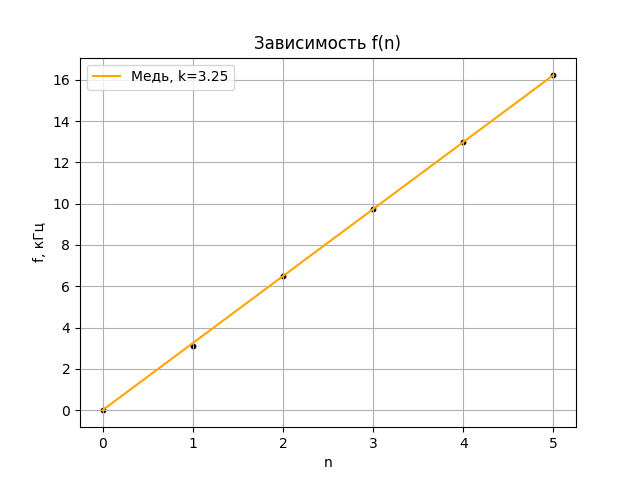
\includegraphics[width=1\linewidth]{graphs/figure1.png}
        \caption{График зависимости частоты акуст. колеб f(n) для меди}
    \end{figure}

    \begin{figure}[H]
        \centering
        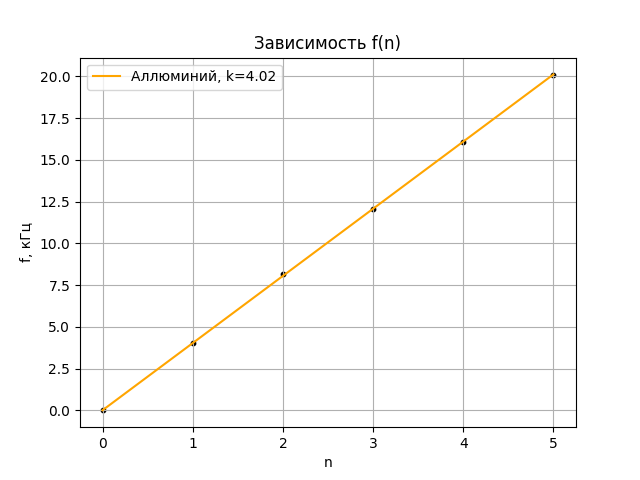
\includegraphics[width=1\linewidth]{graphs/figure2.png}
        \caption{График зависимости частоты акуст. колеб f(n) для аллюминия}
    \end{figure}

    \begin{figure}[H]
        \centering
        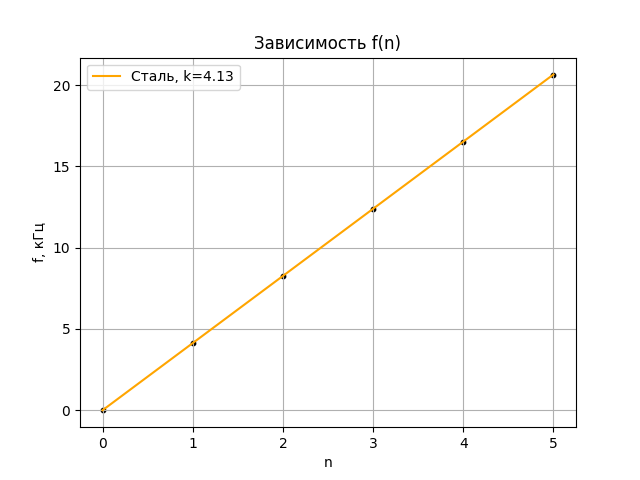
\includegraphics[width=1\linewidth]{graphs/figure3.png}
        \begin{center}
            \caption{График зависимости частоты акуст. колеб f(n) для стали}
        \end{center}
    \end{figure}

    \item По полученным угловым коэффициентам вычислим скорость распространения
    звуковой волны в стержнях, по которой найдем модуль Юнга.
    Случайную погрешность определения углового коэффициента вычисляем как
    \begin{center}
        $\delta^{rand}_k = \sqrt{\frac{1}{N-1}\left(\frac{\langle f^2 \rangle}{\langle n^2 \rangle} - \overline{k}^2\right)}$
    \end{center}
    Тогда относительная погрешность момента инерции: $$\mathcal{E}_{u} = \sqrt{2\left(\frac{\delta_f}{f}\right)^2
     + 2\left(\frac{\delta_L}{L}\right)^2}$$
    А относительная погрешность момента инерции: $$\mathcal{E}_{u} = 2\mathcal{E}_U + \mathcal{E}_f$$
    \begin{table}[h]
        \centering
        \caption{Рассчитанные угловые коэффициенты, скорости аккустической волны, модули Юнга}
        \begin{tabular}{|c|c|c|c|}
        \hline
                     & Медь    & Алюминий & Сталь   \\ \hline
        $k$, кГц     & 3.25    & 4.02        & 4.13 \\ \hline
        $U$, м/с     & 3900    & 4824        & 4956    \\ \hline
        $E$, ГПа     & 137.1     & 64.3      & 191.1     \\ \hline
        $\epsilon_k$ & 0.0010  & 0.0008      & 0.0005  \\ \hline
        $\epsilon_U$ & 0.0011  & 0.0009      & 0.0006  \\ \hline
        $\epsilon_E$ & 0.02    & 0.02        & 0.02    \\ \hline
        \end{tabular}
    \end{table}
    Таким образом, получаем итоговый результат:
    $$ E_{\text{мед}} = (137.1\pm2.7)\;\text{ГПа}, $$
    $$ E_{\text{ал}}  = (64.3\pm1.3)\;\text{ГПа}, $$
    $$ E_{\text{ст}}   = (191.1\pm3.8)\;\text{ГПа} $$
\end{enumerate}

\section{Добротность колебательной системы}
 Проведем дополнительные измерения в окрестности 1-го резонанса
для меди, чтобы получить добротность:
\begin{table}[h]
    \centering
    \caption{\textit{АЧХ}}
    \label{tab:my_label}
    \begin{tabular}{|c|c|c|}
    \hline
    № & Амплитуда, кл & f, КГц \\ \hline
    \multicolumn{3}{c}{идеальный случай $(A_{max})$} \\ \hline
    1 & 8 & 4.2527 \\ \hline
    \multicolumn{3}{c}{увеличение частоты} \\ \hline
    2 & 6 & 4.2537 \\ \hline
    4 & 4 & 4.2543 \\ \hline
    5 & 2 & 4.2572 \\ \hline
    \multicolumn{3}{c}{уменьшение частоты} \\ \hline
    6 & 6 & 4.2523 \\ \hline
    7 & 4 & 4.2513 \\ \hline
    8 & 2 & 4.2489 \\ \hline
    \end{tabular}
\end{table}
Если по точкам прикинуть примерно график и найти частоты на которых $A = \frac{A_{max}}{\sqrt{2}}, \text{то разница между частотами будет } \Delta f = \approx 2~\text{Гц}$
В таком случае добротность можно вычислить следующим образом: $$ Q = \frac{f(A_{max})}{\Delta f} \approx 2000 $$
\begin{figure}[H]
    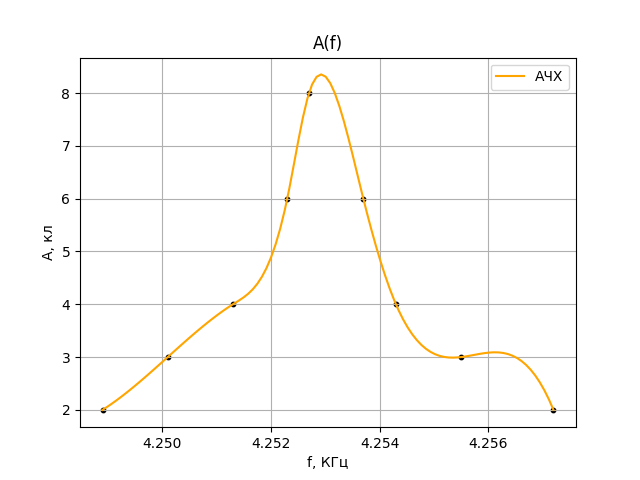
\includegraphics[width=1\linewidth]{graphs/figure4.png}
    \caption{Амплитудно-частотная характеристика системы (зависимость клеток на
    экране осциллографа от подаваемой частоты)}
\end{figure} 

\section{Обсуждение результатов}
В результате работы мы:
\begin{itemize}
    \item Нашли добротность медного стержня как колебательной системы.

    \item Получили зависимость $f(n)$. Как нетрудно убедиться по рис. 2 -- 4,
    во всех случаях аппроксимация прямой действительно применима, причем с очень
    хорошей точностью.

    \item Так как наше теоретическое предположение выполнилось, на его основе
    вычислили скорость звуковой волны во всех данных материалах.

    \item Получили следующие модули Юнга для меди, алюминия и стали:
    $$ E_{\text{мед}} = (137.1\pm2.7)\;\text{ГПа}, $$
    $$ E_{\text{ал}}  = (64.3\pm1.3)\;\text{ГПа}, $$
    $$ E_{\text{ст}}   = (191.1\pm3.8)\;\text{ГПа} $$
\end{itemize}
\end{document}